\lecture{1}{Mon 03 Feb 2025 10:00}{Introduction and Fundamentals}

This is the first lecture. Below are examples of all the environments and
features available in this template.

% =============================================================================
% SECTION 1: Theorem-like environments
% =============================================================================
\section{Basic Structures}

\begin{definition}
    A \textbf{group} is a set $G$ together with a binary operation
    $\cdot : G \times G \to G$ satisfying:
    \begin{enumerate}
        \item \emph{Associativity:} $(a \cdot b) \cdot c = a \cdot (b \cdot c)$ for all $a, b, c \in G$.
        \item \emph{Identity:} There exists $e \in G$ such that $e \cdot a = a \cdot e = a$ for all $a \in G$.
        \item \emph{Inverses:} For each $a \in G$, there exists $a^{-1} \in G$ such that $a \cdot a^{-1} = a^{-1} \cdot a = e$.
    \end{enumerate}
\end{definition}

\begin{theorem}
    Let $G$ be a group. Then the identity element is unique and every element
    has a unique inverse.
\end{theorem}

\begin{proof}
    Suppose $e$ and $e'$ are both identity elements. Then
    \[
        e = e \cdot e' = e'
    \]
    so $e = e'$. For uniqueness of inverses, suppose $b$ and $c$ are both
    inverses of $a$. Then
    \[
        b = b \cdot e = b \cdot (a \cdot c) = (b \cdot a) \cdot c = e \cdot c = c. \qedhere
    \]
\end{proof}

\begin{lemma}
    For any group $G$ and $a, b \in G$, we have $(a \cdot b)^{-1} = b^{-1} \cdot a^{-1}$.
\end{lemma}

\begin{prop}
    Every group of order $p$ (where $p$ is prime) is cyclic.
\end{prop}

\begin{corollary}
    Every group of prime order is abelian.
\end{corollary}

% =============================================================================
% SECTION 2: Non-boxed environments
% =============================================================================
\section{Examples and Remarks}

\begin{eg}
    The integers $\Z$ under addition form a group with identity $0$.
    The rationals $\Q \setminus \{0\}$ under multiplication form a group.
\end{eg}

\begin{remark}
    Not every set with a binary operation is a group. The natural numbers $\N$
    under addition do not form a group because there are no inverses.
\end{remark}

\begin{note}
    Throughout this course, we write $ab$ instead of $a \cdot b$ when the
    operation is clear from context.
\end{note}

\begin{notation}
    We write $|G|$ for the order (number of elements) of a finite group $G$.
\end{notation}

\begin{intuition}
    Think of a group as a set of symmetries. The group operation is composition,
    the identity is ``do nothing,'' and inverses undo transformations.
\end{intuition}

% =============================================================================
% SECTION 3: Math showcase
% =============================================================================
\section{Mathematical Typesetting}

Here are examples of common math constructs:

\textbf{Aligned equations:}
\begin{align}
    \sum_{k=1}^{n} k &= \frac{n(n+1)}{2} \\
    \sum_{k=1}^{n} k^2 &= \frac{n(n+1)(2n+1)}{6} \\
    \sum_{k=1}^{n} k^3 &= \left(\frac{n(n+1)}{2}\right)^2
\end{align}

\textbf{Cases:}
\[
    |x| = \begin{cases}
        x  & \text{if } x \geq 0 \\
        -x & \text{if } x < 0
    \end{cases}
\]

\textbf{Matrices:}
\[
    A = \begin{pmatrix}
        a_{11} & a_{12} & \cdots & a_{1n} \\
        a_{21} & a_{22} & \cdots & a_{2n} \\
        \vdots & \vdots & \ddots & \vdots \\
        a_{m1} & a_{m2} & \cdots & a_{mn}
    \end{pmatrix}
\]

\textbf{Commutative diagram} (using \texttt{tikz-cd}):
\[
    \begin{tikzcd}
        A \arrow[r, "f"] \arrow[d, "g"'] & B \arrow[d, "h"] \\
        C \arrow[r, "k"']                & D
    \end{tikzcd}
\]

\textbf{Number sets:} $\N \subset \Z \subset \Q \subset \R \subset \C$

\textbf{Contradiction:} Assume $\sqrt{2} \in \Q$. Then \ldots\ which gives a
contradiction~\contra.

\textbf{Corrections:} We wrote $1 + 1 = \correct{3}{2}$.

% =============================================================================
% SECTION 4: Boxes
% =============================================================================
\section{Special Boxes}

\begin{correction}
    In the previous lecture we incorrectly stated that every subgroup of a
    non-abelian group is non-abelian. In fact, every group has at least two
    abelian subgroups: $\{e\}$ and any cyclic subgroup.
\end{correction}

\begin{notebox}{Warning}
    The converse of Lagrange's theorem does not hold in general. Not every
    divisor of $|G|$ corresponds to a subgroup of $G$.
\end{notebox}

\begin{important}{Key Result}
    \textbf{Cauchy's Theorem:} If $p$ is a prime dividing $|G|$, then $G$
    contains an element of order $p$.
\end{important}

% =============================================================================
% SECTION 5: TikZ diagrams
% =============================================================================
\section{Diagrams with TikZ}

\textbf{Function graph:}
\begin{center}
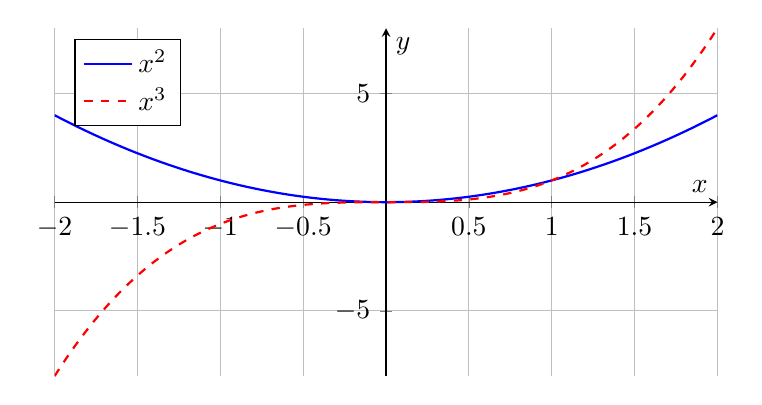
\begin{tikzpicture}
    \begin{axis}[
        axis lines=middle,
        xlabel={$x$},
        ylabel={$y$},
        domain=-2:2,
        samples=100,
        width=10cm,
        height=6cm,
        grid=major,
        legend pos=north west,
    ]
        \addplot[blue, thick]{x^2};
        \addplot[red, thick, dashed]{x^3};
        \legend{$x^2$, $x^3$}
    \end{axis}
\end{tikzpicture}
\end{center}

\textbf{Geometric figure:}
\begin{center}
\begin{tikzpicture}[scale=1.5]
    % Triangle
    \coordinate[label=below left:$A$]  (A) at (0,0);
    \coordinate[label=below right:$B$] (B) at (4,0);
    \coordinate[label=above:$C$]       (C) at (1.5,3);

    \draw[thick] (A) -- (B) -- (C) -- cycle;

    % Midpoints
    \coordinate (MAB) at ($(A)!0.5!(B)$);
    \coordinate (MBC) at ($(B)!0.5!(C)$);
    \coordinate (MAC) at ($(A)!0.5!(C)$);

    % Medians
    \draw[blue, thick] (A) -- (MBC);
    \draw[blue, thick] (B) -- (MAC);
    \draw[blue, thick] (C) -- (MAB);

    % Centroid
    \coordinate (G) at ($(A)!1/3!($(MBC)$)$);
    \fill[red] (G) circle (2pt) node[right] {$G$};

    % Right angle mark at A (if it were a right angle)
    \draw[thick, ->] (-0.5, 0) -- (4.5, 0) node[right] {};
    \draw[thick, ->] (0, -0.3) -- (0, 3.5) node[above] {};
\end{tikzpicture}
\end{center}

\textbf{Vector field sketch:}
\begin{center}
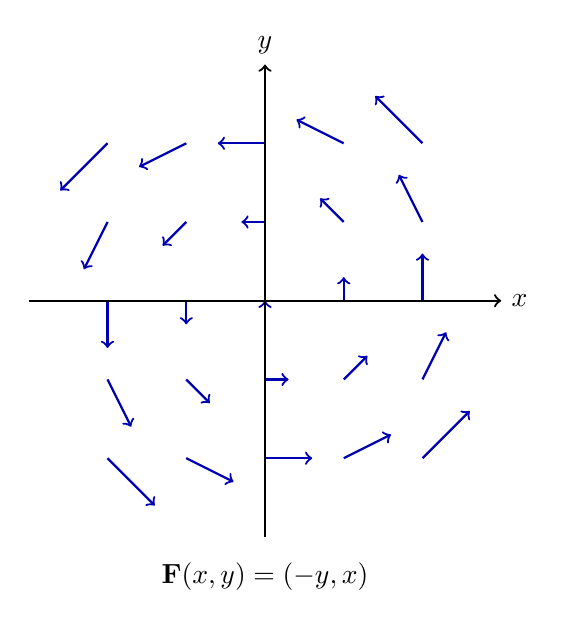
\begin{tikzpicture}
    \foreach \x in {-2,-1,0,1,2} {
        \foreach \y in {-2,-1,0,1,2} {
            \pgfmathsetmacro{\vx}{-\y*0.3}
            \pgfmathsetmacro{\vy}{\x*0.3}
            \draw[->, blue!70!black, thick]
                (\x,\y) -- +(\vx,\vy);
        }
    }
    \draw[thick, ->] (-3,0) -- (3,0) node[right] {$x$};
    \draw[thick, ->] (0,-3) -- (0,3) node[above] {$y$};
    \node at (0, -3.5) {$\mathbf{F}(x,y) = (-y, x)$};
\end{tikzpicture}
\end{center}

\textbf{Commutative diagram (more complex):}
\[
    \begin{tikzcd}[row sep=large, column sep=large]
        \pi_1(X) \arrow[r, "\phi_*"] \arrow[d, "p_*"'] &
        \pi_1(Y) \arrow[d, "q_*"] \\
        H_1(X;\Z) \arrow[r, "\phi_*"'] &
        H_1(Y;\Z)
    \end{tikzcd}
\]

% =============================================================================
% SECTION 6: Inkscape figures (placeholder)
% =============================================================================
\section{Inkscape Figures}

To include an Inkscape figure, place the \texttt{.svg} file in the
\texttt{figures/} directory and use:

\begin{verbatim}
\begin{figure}[ht]
    \centering
    \incfig{my-figure-name}
    \caption{Description of the figure.}
    \label{fig:my-figure-name}
\end{figure}
\end{verbatim}

See the README for full Inkscape workflow instructions.
